%Chapter 7

\chapter{The Deep Quality-Value Learning Family of Algorithms} % Chapter title
\label{ch:dqv_family_of_algorithms} % For referencing the chapter elsewhere, use \autoref{ch:introduction} 


\begin{remark}{Contributions and Outline}
	In the second part of this thesis we have thoroughly studied the level of transferability of deep neural networks that get trained in a supervised learning fashion. From the results of our studies we concluded that significant benefits can come from using pre-trained models over networks that get trained from scratch, and that transfer learning can be a valuable machine learning paradigm for studying the generalization properties of neural networks. In this third, last part of this dissertation we will study whether adopting transfer learning strategies can be as useful in a Deep Reinforcement Learning (DRL) context, where convolutional neural networks get trained for solving optimal control problems. Before studying such transfer learning properties, however, we will start by contributing to the DRL literature by introducing a novel family of DRL algorithms. Therefore, this chapter does not study DRL algorithms from a transfer learning perspective yet, but rather introduces some novel techniques whose transfer learning properties will be researched in the next chapter.
	The structure of this chapter is the following: in Sec. \ref{sec:ijcnn_introduction} we remind the reader with some background information about the field of DRL and recall the mathematical notation that will be used throughout this chapter. In Sec. \ref{sec:dqv_family} we introduce the main algorithmic contributions of our research: a novel family of DRL algorithms the performance of which is thoroughly studied from different perspectives in Sec. \ref{sec:ijcnn_results}. The chapter ends with Sec. \ref{sec:ijcnn_additional_studies} and Sec. \ref{sec:ijcnn_discussion} where we provide a set of additional studies that characterize the performance of our newly introduced algorithms further, and critically discuss their properties. 
\vspace{5mm}

This chapter combines the work presented in the following publications: \citet{sabatelli2018deepqv}, \citet{sabatelli2019approximating}, and \citet{sabatelli2020deep}
\end{remark}

\section{Motivation}
\label{sec:ijcnn_introduction}

In Chapter \ref{ch:reinforcement_learning} we have seen that the aim of value-based Reinforcement Learning (RL) is to construct algorithms which learn value functions that are either able to estimate how good or bad it is for an agent to be in a particular state, or how good it is for an agent to perform a particular action in a given state. Such functions are respectively denoted as the state-value function $V(s)$, and the state-action value function $Q(s,a)$ \cite{sutton2018reinforcement}. We have then seen that in Deep Reinforcement Learning (DRL) the aim is to approximate these value functions with e.g., deep convolutional neural networks \cite{lecun2015deep}, as these kind of networks can serve as universal function approximators as well as powerful feature extractors. Classic model-free RL algorithms like Q-Learning \cite{watkins1992q}, Double Q-Learning \cite{hasselt2010double} and SARSA \cite{rummery1994line} have all led to the development of a ``deep'' version of themselves in which the original RL update rules are expressed as objective functions that can be minimized by gradient descent \cite{mnih2015human, van2016deep, zhao2016deep}. Despite their successful applications \cite{li2017deep}, however, the aforementioned algorithms only aim at approximating the $Q$ function, while completely ignoring the $V$ function, which is an approach that is prone to issues that go back to standard RL literature. As shown by \citet{van2016deep} the DQN algorithm \cite{mnih2015human} is known to overestimate the values of the $Q$ function and requires an additional target network to not diverge (which role, as shown by \citet{achiam2019towards}, is not yet fully understood). These overestimations can partially be corrected by the DDQN \cite{van2016deep} algorithm (see Sec. \ref{sec:deep_reinforcement_learning} of Chapter \ref{ch:reinforcement_learning}), which, despite yielding stability improvements, does not always prevent its $Q$ networks from diverging \cite{van2018deep_triad} and sometimes even underestimating the $Q$ function. Furthermore, DRL algorithms are also extremely slow to train. In what follows, we introduce a new family of DRL algorithms based on the key idea of simultaneously learning the $V$ function alongside the $Q$ function with two separate neural networks. Our main insight is that by jointly approximating the $V$ function and the $Q$ function, the task of learning one of these value functions can be sped up if the model that is responsible for learning it, can rely on what is being learned by the model responsible for learning the other value function. We show that this simple, yet effective idea yields faster, more robust and better model-free Deep Reinforcement Learning.


\section{A Novel Family of Deep Reinforcement Learning Algorithms}
\label{sec:dqv_family}

Just as much as DQN and DDQN are based on two tabular RL algorithms, so is the new family of algorithms presented in this chapter. More specifically we extend two RL algorithms which were first introduced by \citet{wiering2005qv} and then extended by \citet{wiering2009qv} to the use of deep neural networks that serve as function approximators. Training these algorithms robustly is done by taking advantage of some of the techniques which have been reviewed in Chapter \ref{ch:reinforcement_learning}.

\subsection{DQV-Learning}
Our first contribution is the Deep Quality-Value (DQV) Learning algorithm, a novel DRL algorithm which aims at jointly approximating the $V$ function alongside the $Q$ function in an \textcolor{RoyalBlue}{on-policy} learning setting. This algorithm is based on the QV($\lambda$) algorithm \cite{wiering2005qv}, a tabular RL algorithm which was reviewed in Chapter \ref{ch:reinforcement_learning} and that learns the $V$ function via the simplest form of TD-Learning \cite{sutton1988learning}. The estimates that are learned by this value function are then used to update the $Q$ function in a Q-Learning resembling way. Specifically, after a RL transition $\langle$ $s_{t}$, $a_{t}$, $r_{t}$, $s_{t+1}$ $\rangle$, QV$(\lambda)$ uses the TD$(\lambda)$ learning rule \cite{sutton1988learning} to update the $V$ function for all states: 
\begin{equation}
V(s):= V(s) + \alpha \big[ r_{t} + \gamma V(s_{t+1}) - V(s_t) \big] e_{t}(s),
\label{eq:qv_lambda_v_update}
\end{equation}
where $\alpha$ stands for the learning rate and $\gamma$ is the discount factor, while $e_t(s)$ are the elibility traces \cite{peng1994incremental, wiering1998speeding, geist2014off} that are necessary for keeping track if a particular state has occurred before a certain time-step or not. These are updated for all states as follows:  
\begin{equation} 
e_{t}(s) = \gamma \lambda e_{t-1}(s) + \eta_t(s),
\end{equation}
where $\eta_t(s)$ is an indicator function that returns a value of $1$ whether a particular state occurred at time $t$ and $0$ otherwise. Before updating the $V$ function, QV$(\lambda)$ updates the $Q$ function first, and does this via the following update rule:
\begin{equation}
Q(s_{t}, a_{t}):= Q(s_{t}, a_{t}) + \alpha \big[r_{t} + \gamma V(s_{t+1}) - Q(s_{t}, a_{t}) \big].
\label{eq:qv_lambda_q_update}
\end{equation}

We take inspiration from this specific learning dynamic and aim at learning an approximation of both the $V$ function, and the $Q$ function, with two neural networks that are respectively parametrized by $\Phi$ and $\theta$. To do so, we follow the same principles which have led to the development of the DQN algorithm. Therefore, starting from Eq. \ref{eq:qv_lambda_v_update}, and after removing $e_{t}(s)$ for simplicity, we get the following objective function which is used by DQV for learning the state-value function:
\begin{multline}
L(\Phi) = \mathds{E}_{\langle s_{t},a_{t},r_{t},s_{t+1}\rangle\sim U(D)} \bigg[\big(r_{t} + \gamma V(s_{t+1}; \Phi^{-}) - V(s_{t}; \Phi)\big)^{2}\bigg],
\label{eq:dqv_v_update}
\end{multline}
while the following loss is minimized for learning the $Q$ function when starting from Eq. \ref{eq:qv_lambda_q_update}:
\begin{multline}
    L(\theta) = \mathds{E}_{\langle s_{t},a_{t},r_{t},s_{t+1}\rangle\sim U(D)} \bigg[\big(r_{t} + \gamma V(s_{t+1}; \Phi^{-}) - Q(s_{t}, a_{t}; \theta)\big)^{2}\bigg],
\label{eq:dqv_q_update}
\end{multline}
where $D$ is the Experience-Replay memory buffer, used for uniformly sampling batches of RL trajectories $\langle s_{t},a_{t},r_{t},s_{t+1}\rangle$, and $\Phi^{-}$ is the target-network used for the construction of the TD-errors. Note that the role of this target network is different from its role within the DQN algorithm reviewed in Chapter \ref{ch:reinforcement_learning}. In DQV, this network corresponds to a copy of the network which approximates the state-value function and not the state-action value function. It is also worth noting that both networks learn from the same TD-target which comes in the following form:
\begin{equation}
y_{t}^{DQV} = r_{t} + \gamma V(s_{t+1}; \Phi^{-}). 
\end{equation}

\subsection{DQV-Learning with Multilayer Perceptrons}
We start by exploring whether this learning dynamic of jointly approximating two value functions simultaneously, and let the $Q$ function bootstrap from the TD-targets that are learned from the $V$ network, can yield successful results on a set of preliminary experiments. To do so, we use two classic control problems that are well known in the RL literature: \texttt{Acrobot} \cite{sutton1996generalization} and \texttt{Cartpole} \cite{barto1983neuronlike} with both environments being provided by the Open-AI Gym package \cite{brockman2016openai}. We approximate the $V$ function and the $Q$ function with a two hidden layer Multilayer Perceptron (MLP) that is activated by a ReLU non linearity ($f(x) = max (0,x)$) and compare the performance of DQV to the one of the DQN and the DDQN algorithms, which use the same MLP but for approximating the $Q$ function only. Given the simplicity of these two control problems we did not integrate DQV with the target network $\Phi^{-}$ yet. Our preliminary results reported in Fig. \ref{fig:mlp_dqv_results}, show the benefits that can come from training two separate networks with the update rules reported in Eq. \ref{eq:dqv_v_update} and Eq. \ref{eq:dqv_q_update}. We can in fact observe that on both control problems DQV-Learning outperforms DQN and DDQN, by converging significantly faster. 

\begin{figure}[ht!]
  \begin{tikzpicture}[scale = 0.65]
      \begin{axis}[
	name=ax1,
      	grid style={dashed,gray},
      	grid = both, 
      	tick style=black,
	title=Acrobot,
        xlabel=Episodes,
        ylabel=Reward,
      ]


      \addlegendentry{DQV}
      \addlegendentry{DQN}
      \addlegendentry{DDQN}
      
      \addplot [ultra thick, red, mark=.] table [y=DQV, x=episodes]
      {./Results/Chapter07/logs/acrobot_results.txt};
      \addplot [ultra thick, blue, mark=.] table [y=DQN, x=episodes]{./Results/Chapter07/logs/acrobot_results.txt};
      \addplot [ultra thick, green, mark=.] table [y=DDQN, x=episodes]{./Results/Chapter07/logs/acrobot_results.txt};
     
      \legend{}

      \end{axis}

      \begin{axis}[
	at={(ax1.south east)},
	xshift=2cm,
      	grid style={dashed,gray},
      	grid = both, 
      	tick style=black,
	title=Cartpole,
        xlabel=Episodes,
        ylabel= Reward,
	legend columns=3, 
        legend style={font=\Large, at={(-0.65,-0.3,-0.4)},anchor=north west,legend columns=3},
      ]

      \addlegendentry{DQV}
      \addlegendentry{DQN}
      \addlegendentry{DDQN}
 
      \addplot [ultra thick, red, mark=.] table [y=DQV, x=episodes]
      {./Results/Chapter07/logs/cartpole_results.txt};
      \addplot [ultra thick, blue, mark=.] table [y=DQN, x=episodes]{./Results/Chapter07/logs/cartpole_results.txt};
      \addplot [ultra thick, green, mark=.] table [y=DDQN, x=episodes]{./Results/Chapter07/logs/cartpole_results.txt};
 
      \end{axis}
	\end{tikzpicture}
	\caption{}
	\label{fig:mlp_dqv_results} 
\end{figure}




\subsection{DQV-Max Learning}
Based on the successful results presented in Fig. \ref{fig:mlp_dqv_results} that highlight the potential benefits that could come from jointly approximating two value functions over one, we now introduce the Deep Quality-Value-Max (DQV-Max) algorithm, a novel DRL algorithm which builds on top of some of the ideas that characterize DQV. Similarly as done for DQV, we still aim at jointly learning an approximation of the $V$ function and the $Q$ function, but in this case, the goal is to do this with an \textcolor{RoyalBlue}{off-policy} learning scheme. To construct this algorithm we take inspiration from the QV-Max RL algorithm introduced by \citet{wiering2009qv}. The key component of QV-Max is the use of the $\underset{a\in \mathcal{A}}{\max}\: Q(s_{t+1}, a)$ operator, which makes RL algorithms learn off-policy. We use this operator when approximating the $V$ function and for computing TD-errors which correspond to the ones that are also used by the DQN algorithm. However, within DQV-Max, these TD-errors are used by the state-value network and not by the state-action value network. This results in the following loss which is used for learning the $V$ function:
\begin{multline}
L(\Phi) = \mathds{E}_{\langle s_{t},a_{t},r_{t},s_{t+1}\rangle\sim U(D)} \bigg[\big(r_{t} + \gamma \: \underset{a\in \mathcal{A}}{\max}\: Q(s_{t+1}, a; \theta^{-}) - V(s_{t}; \Phi)\big)^{2}\bigg].
\label{eq:dqv_max_v}
\end{multline}
In this case the target network $\theta^{-}$ corresponds to the same target network that is also used by DQN. The TD-error $r_{t} + \gamma \: \underset{a\in \mathcal{A}}{\max}\: Q(s_{t+1}, a; \theta^{-})$ is however only used for learning the $V$ function. When it comes to the $Q$ function we use the same update rule that is presented in Eq. \ref{eq:dqv_q_update} with the only difference being that in this case no $\Phi^{-}$ target network is used. Despite requiring the computation of two different targets for learning, we noticed that DQV-Max did not benefit from using two distinct target networks, therefore its loss function for approximating the $Q$ function is simply:
\begin{multline}
    L(\theta) = \mathds{E}_{\langle s_{t},a_{t},r_{t},s_{t+1}\rangle\sim U(D)} \bigg[\big(r_{t} + \gamma V(s_{t+1}; \Phi) - Q(s_{t}, a_{t}; \theta)\big)^{2}\bigg].
    \label{eq:dqv_max_q}
\end{multline}

The pseudocode of both DQV and DQV-Max is presented at the end of this thesis in Algorithm \ref{alg: dqv_algorithms} which can be found in Appendix \ref{ch:appendixDQV}. The pseudocode is an adaptation of a standard DRL training loop which corresponds to what is usually presented within the literature \cite{mnih2015human}. We just make explicit use of the hyperparameters \texttt{total\_a} and \texttt{c} which ensure that enough actions have been performed by the agent before updating the weights of the target network. We also ensure via the hyperparameter \texttt{total\_e}, that enough episodes are stored within the memory buffer (which has capacity $\mathcal{N}$) before starting to optimize the neural networks. 



\section{Results}
\label{sec:ijcnn_results}

\subsection{Global Evaluation}
\label{sec:global_evaluation}

We evaluate the performance of DQV and DQV-Max on a subset of 15 games coming from the popular \texttt{Atari-2600} benchmark \cite{bellemare2013arcade}. Our newly introduced algorithms are compared against DQN and DDQN. To keep all the comparisons as fair as possible we follow the same experimental setup and evaluation protocol which was used in \cite{mnih2015human} and \cite{van2016deep}. The only difference between DQV and DQV-Max, and DQN and DDQN is the exploration schedule which is used. Differently from the latter two algorithms, which use an epsilon-greedy strategy which has an $\epsilon$ starting value of 1.0, DQV and DQV-Max's exploration policy starts with an initial $\epsilon$ value of 0.5. All other hyperparameters, ranging from the size of the Experience-Replay memory buffer to the architectures of the neural networks, are kept the same among all algorithms. We refer the reader to the original DQN paper \cite{mnih2015human} for an in-depth overview of all these hyperparameters. The performance of the algorithms is tested based on the popular \texttt{no-op action} evaluation regime. At the end of the training, the learned policies are tested over a series of episodes for a total amount of 5 minutes of emulator time. All testing episodes start by executing a set of partially random actions to test the level of generalization of the learned policies. We present our results in Table \ref{tab:ch07_results} where the best performing algorithm is reported in a green cell while the second-best performing algorithm is reported in a yellow cell. As is common within the DRL literature, the table also reports the scores which would be obtained by an expert human player and by a random policy. When the scores over games are equivalent, we report in the green and yellow cells the fastest and second fastest algorithm with respect to its convergence time (determined by a visual inspection of the learning curves). 

We can start by observing that DQV and DQV-Max successfully master all the environments on which they have been tested, with the only exception being the \texttt{Montezuma's Revenge} game. It is well-known that this game requires more sophisticated exploration strategies than the epsilon-greedy one \cite{fortunato2017noisy}, and was also not mastered by DQN and DDQN when these algorithms were introduced. We can also observe that there is no algorithm which performs best on all the tested environments even though, as highlighted by the green and yellow cells, the algorithms of the DQV-family seem to generally perform better than DQN and DDQN, with DQV-Max being the overall best performing algorithm in our set of experiments. When either DQV or DQV-Max are not the best performing algorithm (see for example the \texttt{Boxing} and \texttt{Crazy Climber} environments), we can still observe that our algorithms managed to converge to a policy which is not significantly worst than the one learned by DQN and DDQN.
There is however one exception being the \texttt{Road Runner} environment. In fact, in this game, DDQN significantly outperforms DQV and DQV-Max. It is also worth noting the results on the \texttt{Bank Heist} and \texttt{Enduro} environments. Both DQN and DDQN failed to achieve super-human performance on these games, while DQV and DQV-Max successfully managed to obtain a significantly higher score than the one obtained by a professional human player. On the \texttt{Bank Heist} environment DQV and DQV-Max obtain $\approx 400$ points more than an expert human player, while on the \texttt{Enduro} environment their performance is almost three times better than the one obtained by DQN and DDQN.

\begin{table*}[ht]
\caption{The results obtained by DQV and DQV-Max on a subset of 15 \texttt{Atari} games, compared with those obtained by DQN and DDQN (reproduced from their corresponding publications). We can see that our newly introduced algorithms have a comparable, and often even better performance than DQN and DDQN. As highlighted by the green cells the overall best performing algorithm in our set of experiments is DQV-Max while the second-best performing algorithm is DQV (as reported by the yellow cells). Specific attention should be given to the games \texttt{BankHeist} and \texttt{Enduro} where DQV and DQV-Max are the only algorithms which can master the game with a final super-human performance.}
\centering
\resizebox{\columnwidth}{!}{%
\begin{tabular}{l|r|r|r|r|r|r}
\hline 
Environment & Random & Human & DQN \cite{mnih2015human} & DDQN \cite{van2016deep} & DQV & DQV-Max\\
\hline \hline
\texttt{Asteroids} &719.10 &13156.70 &\cellcolor{yellow!25}1629.33 &930.60 &1445.40 & \cellcolor{green!25}1846.08\\
\texttt{Bank Heist} &14.20 & 734.40 & 429.67 & 728.30 & \cellcolor{green!25}1236.50 & \cellcolor{yellow!25}1118.28 \\
\texttt{Boxing} &0.10 & 4.30 & 71.83 & \cellcolor{green!25}81.70 & 78.66 & \cellcolor{yellow!25}{80.15} \\
\texttt{Crazy Climber} &10780.50 & 35410.50 & \cellcolor{green!25}114103.33 & 101874.00 & \cellcolor{yellow!25}108600.00 & 1000131.00\\
\texttt{Enduro} &0.00 & 309.60 & 301.77 & 319.50 & \cellcolor{yellow!25}829.33 & \cellcolor{green!25}875.64 \\
\texttt{Fishing Derby} &-91.70 & 5.50 & -0.80 & \cellcolor{yellow!25}20.30 & 1.12 & \cellcolor{green!25}20.42  \\
\texttt{Frostbite} &65.20 & 4334.70 & \cellcolor{green!25}328.33 & 241.50 & 271.86 & \cellcolor{yellow!25}281.36 \\
\texttt{Gopher} &257.60 & 2321.00 &\cellcolor{green!25}{8520.00} &8215.40 &\cellcolor{yellow!25}{8230.30} &7940.00 \\
\texttt{Ice Hockey} &-11.20 & 0.90 & \cellcolor{yellow!25}-1.60 & -2.40 & -1.88 & \cellcolor{green!25}-1.12\\
\texttt{James Bond} &29.00 & 406.70 & \cellcolor{green!25}{576.67} & 438.00 & 372.41 & \cellcolor{yellow!25}{440.80} \\
\texttt{Montezuma's Revenge} &0.00 & 4366.70 & 0.00 & 0.00 & 0.00 & 0.00\\
\texttt{Ms.Pacman} &307.30 & 15693.40 & 2311.00 & 3210.00 & \cellcolor{green!25}3590.00 & \cellcolor{yellow!25}3390.00\\
\texttt{Pong} &-20.70 &9.30 & 18.90 & 21.00 & \cellcolor{yellow!25}21.00 & \cellcolor{green!25}21.00\\
\texttt{Road Runner} &11.50 &7845.00 &18256.67  &\cellcolor{green!25}48377.00  &\cellcolor{yellow!25}39290.00  & 20700.00\\
\texttt{Zaxxon} &32.50 &9173.30 &4976.67  &\cellcolor{yellow!25}10182.00  &\cellcolor{green!25}10950.00  & 8487.00\\

\end{tabular}%
}
\label{tab:ch07_results}
\end{table*}



\subsection{Convergence Time}
\label{sec:convergence_time}

While DRL algorithms have certainly obtained impressive results on the \texttt{Atari-2600} benchmark, it is also true that the amount of training time which is required by these algorithms can be very long. Over the years, several techniques reviewed in Sec. \ref{sec:deep_reinforcement_learning} of Chapter \ref{ch:reinforcement_learning}, ranging from Prioritized Experience Replay (PER) \cite{wang2016dueling} to the Rainbow extensions introduced by \citet{hessel2018rainbow}, have been proposed to reduce the training time of DRL algorithms. It is therefore natural to investigate whether jointly approximating the $V$ function alongside the $Q$ function can lead to significant benefits in this behalf. Unlike the $Q$ function
    \begin{align*}
	     Q^{\pi}(s,a)=\mathds{E}\bigg[\sum_{k=0}^{\infty}\gamma^{k}r_{t+k} \bigg| s_t = s, a_t=a, \pi\bigg],
    \end{align*}
recall that the state-value function
  \begin{align*}
	    V^{\pi}(s)=\mathds{E}\bigg[\sum_{k=0}^{\infty}\gamma^{k}r_{t+k}\bigg| s_t = s, \pi \bigg],
    \end{align*}
 is not conditioned on the set of possible actions that the agent may take, and therefore requires fewer parameters to converge. Since DQV and DQV-Max use the estimates of the $V$ network to train the $Q$ function, it is possible that the $Q$ function could directly benefit from these estimates and as a result converge faster than when regressed towards itself (as happens in DQN).

We use two self-implemented versions of DQN and DDQN for comparing the convergence time that is required during training by all the tested algorithms on three increasingly complex \texttt{Atari} games: \texttt{Boxing, Pong} and \texttt{Enduro}. Our results, reported in Fig. \ref{fig:ch07_convergence_results}, show that DQV and DQV-Max converge significantly faster than DQN and DDQN, therefore confirming the preliminary results which we reported in Fig. \ref{fig:mlp_dqv_results}, and highlighting once again the benefits of jointly approximating two value functions instead of one when it comes to the overall convergence time that is required by the algorithms. Even though, as presented in Table \ref{tab:ch07_results}, DQV and DQV-Max do not always significantly outperform DQN and DDQN in terms of the final cumulative reward which is obtained, it is worth noting that these algorithms require significantly less training episodes to converge on all tested games. This benefit makes our two novel algorithms faster alternatives within model-free DRL.

\begin{figure}[ht!]
  \begin{tikzpicture}[scale = 0.65]
      \begin{axis}[
	name=ax1,
      	grid style={dashed,gray},
      	grid = both, 
      	tick style=black,
	title=Boxing,
        xlabel=Episodes,
        ylabel=Reward,
      ]


      \addlegendentry{DQV} 
      \addlegendentry{DQV-Max}  
      \addlegendentry{DQN}
      \addlegendentry{DDQN}
      
      \addplot [ultra thick, red, mark=.] table [y=DQV, x=episodes]
      {./Results/Chapter07/logs/boxing_results.txt};
       \addplot [ultra thick, yellow, mark=.] table [y=DQV-Max, x=episodes]
      {./Results/Chapter07/logs/boxing_results.txt};
      \addplot [ultra thick, blue, mark=.] table [y=DQN, x=episodes]{./Results/Chapter07/logs/boxing_results.txt};
      \addplot [ultra thick, green, mark=.] table [y=DDQN, x=episodes]{./Results/Chapter07/logs/boxing_results.txt};
     
      \legend{}

      \end{axis}

      \begin{axis}[
      	at={(ax1.south east)},
	xshift=2cm,
	grid style={dashed,gray},
      	grid = both, 
      	tick style=black,
	title=Enduro,
        xlabel=Episodes,
        ylabel=Reward,
      ]


      \addlegendentry{DQV} 
      \addlegendentry{DQV-Max}  
      \addlegendentry{DQN}
      \addlegendentry{DDQN}
      
      \addplot [ultra thick, red, mark=.] table [y=DQV, x=episodes]
      {./Results/Chapter07/logs/enduro_results.txt};
       \addplot [ultra thick, yellow, mark=.] table [y=DQV-Max, x=episodes]
      {./Results/Chapter07/logs/enduro_results.txt};
      \addplot [ultra thick, blue, mark=.] table [y=DQN, x=episodes]{./Results/Chapter07/logs/enduro_results.txt};
      \addplot [ultra thick, green, mark=.] table [y=DDQN, x=episodes]{./Results/Chapter07/logs/enduro_results.txt};
     
      \legend{}

      \end{axis}


      \begin{axis}[
	at={(ax1.south east)},
	xshift=-2cm,
      	yshift=-8cm,
	grid style={dashed,gray},
      	grid = both, 
      	tick style=black,
	title=Pong,
        xlabel=Episodes,
        ylabel= Reward,
	legend columns=4, 
        legend style={font=\Large, at={(-0.3,-0.3,-0.4)},anchor=north west,legend columns=3},
      ]


	\addlegendentry{DQV} 
	\addlegendentry{DQV-Max}  
	\addlegendentry{DQN}
	\addlegendentry{DDQN}

      \addplot [ultra thick, red, mark=.] table [y=DQV, x=episodes]
      {./Results/Chapter07/logs/pong_results.txt};
      \addplot [ultra thick, yellow, mark=.] table [y=DQV-Max, x=episodes]
      {./Results/Chapter07/logs/pong_results.txt};
      
      \addplot [ultra thick, blue, mark=.] table [y=DQN, x=episodes]{./Results/Chapter07/logs/pong_results.txt};
      \addplot [ultra thick, green, mark=.] table [y=DDQN, x=episodes]{./Results/Chapter07/logs/pong_results.txt};
 
      \end{axis}
	\end{tikzpicture}
	\caption{Learning curves obtained during training on three different \texttt{Atari} games by DQV and DQV-Max, and DQN and DDQN. We can observe that on these games both DQV and DQV-Max converge significantly faster than DQN and DDQN and that they obtain higher cumulative rewards on the \texttt{Enduro} environment.}
	\label{fig:ch07_convergence_results} 
\end{figure}



\subsection{Quality of the Learned Value Functions}
\label{sec:quality_of_value_functions}

It is well-known that the combination of RL algorithms with function approximators can yield DRL algorithms that diverge. The popular Q-Learning algorithm is known to result in unstable learning both if linear \cite{tsitsiklis1997analysis} and non-linear functions are used when approximating the $Q$ function \cite{van2018deep_triad}. As seen at the end of Chapter \ref{ch:reinforcement_learning}, this divergence according to \citet{sutton2018reinforcement} is caused by the interplay of three elements that are known as the \textit{`Deadly Triad'} of DRL. The elements of this triad are:
\begin{itemize}
    \item \textit{a function approximator}: which is used for learning an approximation of a value function that could not be learned in the tabular RL setting due to a too large state-action space.
    \item \textit{bootstrapping}: when the algorithms use a future estimated value for learning the same kind of estimate.
    \item \textit{off-policy learning}: when a future estimated value is different from the one which would be computed by the policy the agent is following.
\end{itemize}{}

\citet{van2018deep_triad} have shown that the \textit{`Deadly Triad'} is responsible for enhancing one of the most popular biases that characterize the Q-Learning algorithm: the overestimation bias of the $Q$ function \cite{hasselt2010double}. It is therefore natural to study how DQV and DQV-Max relate to the \textit{`Deadly Triad'} of DRL, and to investigate up to what extent these algorithms suffer from the overestimation bias of the $Q$ function. To do this we monitor the estimates that are given by the network that is responsible for approximating the $Q$ function. More specifically, at training time, we compute the averaged $\underset{a \in \cal A}{\max}\:Q(s_{t+1}, a)$ over a set ($n$) of full evaluation episodes as defined by 
\begin{equation}
\frac{1}{n}\sum_{t=1}^{n}\underset{a \in \cal A}{\max}\:Q(s_{t+1}, a;\theta).
\end{equation}
As suggested by \citet{van2016deep} these estimates can then be compared to the averaged discounted return of all visited states that comes from an agent that has already concluded training. By analyzing whether the $Q$ values which are estimated while training differ from the ones which should be predicted by the end of it, it is possible to quantitatively characterize the level of divergence of DRL algorithms. We report our results in Figs. \ref{fig:overestimation_bias_results_dqn}, \ref{fig:overestimation_bias_results_ddqn}, \ref{fig:overestimation_bias_results_dqv} and \ref{fig:overestimation_bias_results_dqv_max} where the black full lines correspond to the value estimates that come from each algorithm at training time, while the coloured lines correspond to the actual averaged discounted return that is given by an already trained agent.


We can start by observing that the values denoting the averaged discounted return obtained by each algorithm differ among agents. This is especially the case when it comes to the \texttt{Enduro} environment, and is a result which is in line with what has been presented in Table \ref{tab:results}: DQV and DQV-Max lead to better final policies than DQN and DDQN. Furthermore, when we compare these baseline values to the value estimates that are obtained during training, we can observe that the ones obtained by the DQN algorithm significantly diverge from the ones which should be predicted by the end of training. This behavior is known to be caused by the overestimation bias of the $Q$ function which can be corrected by the DDQN algorithm. By analyzing the value estimates of DQV and DQV-Max we can observe that both algorithms produce value estimates which are more similar to the ones computed by DDQN than to the ones given by DQN. This is especially the case for DQV (Fig. \ref{fig:overestimation_bias_results_dqv}). In fact, its value estimates nicely correspond to the averaged discounted return baseline, both on the \texttt{Pong} environment and on the \texttt{Enduro} environment. The estimates coming from DQV-Max, however, seem to diverge more when compared to DQV and DDQN's ones. This is clearer on the \texttt{Enduro} environment, where the algorithm does show some divergence (right plot of Fig. \ref{fig:overestimation_bias_results_dqv_max}). However, we can also observe that this divergence is less strong when compared to DQN's one. The value estimates of the latter algorithm keep growing over time, while DQV-Max's ones get bounded while training progresses (see the two right plots of Fig. \ref{fig:overestimation_bias_results_dqn} and Fig. \ref{fig:overestimation_bias_results_dqv_max}). This results in smaller estimated $Q$ values. We believe that there are mainly two reasons why our algorithms suffer less from the overestimation bias of the $Q$ function. When it comes to DQV, we believe that this algorithm suffers less from this bias since it is an on-policy learning algorithm. Such algorithms are trained on exploration actions with lower $Q$ values. Because of its \textit{on-policy} learning scheme, DQV also does not present one element of the \textcolor{RoyalBlue}{`Deadly Triad'}, which might help reducing divergence. When it comes to DQV-Max, we believe that the reason why this algorithm does not diverge as much as DQN can be found in the way it approximates the $Q$ function. One key component of the \textit{`Deadly Triad'}, is that divergence occurs if the $Q$ function is learned by regressing towards itself. As given by Eq. \ref{eq:dqv_max_q} we can see that this does not hold for DQV-Max, since the $Q$ function bootstraps with respect to estimates that come from the $V$ network. We believe that this specific learning dynamic, which also holds for the DQV algorithm, makes our algorithms less prone to estimate large $Q$ values.

% add overestimation bias results
\begin{figure}[ht!]
  \begin{tikzpicture}[scale = 0.65]
      \begin{axis}[
	name=ax1,
      	grid style={dashed,gray},
      	grid = both, 
      	tick style=black,
	title=Pong,
        xlabel=Training Steps,
        ylabel=Value Estimates,
      ]


      \addlegendentry{DQN-True Value}
      \addlegendentry{DQN-Estimated Value}
      
      \addplot [ultra thick, black, mark=.] table [y=true_return_DQN, x=training_steps]
      {./Results/Chapter07/logs/overestimation_pong.txt};
      \addplot [ultra thick, blue, mark=.] table [y=estimate_DQN, x=training_steps]{./Results/Chapter07/logs/overestimation_pong.txt};
     
      \legend{}

      \end{axis}

      \begin{axis}[
	at={(ax1.south east)},
	xshift=2cm,
      	grid style={dashed,gray},
      	grid = both, 
      	tick style=black,
	title=Enduro,
        xlabel=Training Steps,
        ylabel= Value Estimates,
	legend columns=3, 
        legend style={font=\Large, at={(-0.85,-0.3,-0.4)},anchor=north west,legend columns=3},
      ]

      \addlegendentry{DQN-True Value}
      \addlegendentry{DQN-Estimated Value}

      \addplot [ultra thick, black, mark=.] table [y=true_return_DQN, x=training_steps]
      {./Results/Chapter07/logs/overestimation_enduro.txt};
      \addplot [ultra thick, blue, mark=.] table [y=estimate_DQN, x=training_steps]{./Results/Chapter07/logs/overestimation_enduro.txt};
 
      \end{axis}
	\end{tikzpicture}
	\caption{}
	\label{fig:overestimation_bias_results} 
\end{figure}


\begin{figure}[ht!]
  \begin{tikzpicture}[scale = 0.65]
      \begin{axis}[
	name=ax1,
      	grid style={dashed,gray},
      	grid = both, 
      	tick style=black,
	title=Pong,
        xlabel=Training Steps,
        ylabel=Value Estimates,
      ]


      \addlegendentry{DDQN-True Value}
      \addlegendentry{DDQN-Estimated Value}
      
      \addplot [ultra thick, black, mark=.] table [y=true_return_DDQN, x=training_steps]
      {./Results/Chapter07/logs/overestimation_pong.txt};
      \addplot [ultra thick, green, mark=.] table [y=estimate_DDQN, x=training_steps]{./Results/Chapter07/logs/overestimation_pong.txt};
     
      \legend{}

      \end{axis}

      \begin{axis}[
	at={(ax1.south east)},
	xshift=2cm,
      	grid style={dashed,gray},
      	grid = both, 
      	tick style=black,
	title=Enduro,
        xlabel=Training Steps,
        ylabel= Value Estimates,
	legend columns=3, 
        legend style={font=\Large, at={(-0.85,-0.3,-0.4)},anchor=north west,legend columns=3},
      ]

      \addlegendentry{DDQN-True Value}
      \addlegendentry{DDQN-Estimated Value}
      

      \addplot [ultra thick, black, mark=.] table [y=true_return_DDQN, x=training_steps]
      {./Results/Chapter07/logs/overestimation_enduro.txt};
      \addplot [ultra thick, green, mark=.] table [y=estimate_DDQN, x=training_steps]{./Results/Chapter07/logs/overestimation_enduro.txt};
 
      \end{axis}
	\end{tikzpicture}
	\caption{Results investigating the extent to which the DDQN algorithm suffers from the overestimation bias of the $Q$ function. We can observe that compared to the analysis presented in Fig. \ref{fig:overestimation_bias_results_dqn}, the DDQN algorithm prevents its Q-Network from diverging since on both \texttt{Atari} environments the $\underset{a \in \cal A}{\max}\:Q(s_{t+1}, a)$ estimates do not diverge from the observed real return of a trained agent. These results replicate the findings reported by \citet{van2018deep_triad}.}
	\label{fig:overestimation_bias_results_ddqn} 
\end{figure}


\begin{figure}[ht!]
  \begin{tikzpicture}[scale = 0.65]
      \begin{axis}[
	name=ax1,
      	grid style={dashed,gray},
      	grid = both, 
      	tick style=black,
	title=Pong,
        xlabel=Training Steps,
        ylabel=Value Estimates,
      ]


      \addlegendentry{DQV-True Value}
      \addlegendentry{DQV-Estimated Value}
      
      \addplot [ultra thick, black, mark=.] table [y=true_return_DQV, x=training_steps]
      {./Results/Chapter07/logs/overestimation_pong.txt};
      \addplot [ultra thick, red, mark=.] table [y=estimate_DQV, x=training_steps]{./Results/Chapter07/logs/overestimation_pong.txt};
     
      \legend{}

      \end{axis}

      \begin{axis}[
	at={(ax1.south east)},
	xshift=2cm,
      	grid style={dashed,gray},
      	grid = both, 
      	tick style=black,
	title=Enduro,
        xlabel=Training Steps,
        ylabel= Value Estimates,
	legend columns=3, 
        legend style={font=\Large, at={(-0.85,-0.3,-0.4)},anchor=north west,legend columns=3},
      ]

      \addlegendentry{DQV-True Value}
      \addlegendentry{DQV-Estimated Value}

      \addplot [ultra thick, black, mark=.] table [y=true_return_DQV, x=training_steps]
      {./Results/Chapter07/logs/overestimation_enduro.txt};
      \addplot [ultra thick, red, mark=.] table [y=estimate_DQV, x=training_steps]{./Results/Chapter07/logs/overestimation_enduro.txt};
 
      \end{axis}
	\end{tikzpicture}
	\caption{}
	\label{fig:overestimation_bias_results_ddqn} 
\end{figure}


\begin{figure}[ht!]
  \begin{tikzpicture}[scale = 0.65]
      \begin{axis}[
	name=ax1,
      	grid style={dashed,gray},
      	grid = both, 
      	tick style=black,
	title=Pong,
        xlabel=Training Steps,
        ylabel=Value Estimates,
      ]


      \addlegendentry{DQV-Max-True Value}
      \addlegendentry{DQV-Max-Estimated Value}
      
      \addplot [ultra thick, black, mark=.] table [y=true_return_DQV-Max, x=training_steps]
      {./Results/Chapter07/logs/overestimation_pong.txt};
      \addplot [ultra thick, yellow, mark=.] table [y=estimate_DQV-Max, x=training_steps]{./Results/Chapter07/logs/overestimation_pong.txt};
     
      \legend{}

      \end{axis}

      \begin{axis}[
	at={(ax1.south east)},
	xshift=2cm,
      	grid style={dashed,gray},
      	grid = both, 
      	tick style=black,
	title=Enduro,
        xlabel=Training Steps,
        ylabel= Value Estimates,
	legend columns=3, 
        legend style={font=\Large, at={(-1,-0.3,-0.4)},anchor=north west,legend columns=3},
      ]

      \addlegendentry{DQV-Max-True Value}
      \addlegendentry{DQV-Max-Estimated Value}

      \addplot [ultra thick, black, mark=.] table [y=true_return_DQV-Max, x=training_steps]
      {./Results/Chapter07/logs/overestimation_enduro.txt};
      \addplot [ultra thick, yellow, mark=.] table [y=estimate_DQV-Max, x=training_steps]{./Results/Chapter07/logs/overestimation_enduro.txt};
 
      \end{axis}
	\end{tikzpicture}
	\caption{Results investigating the extent to which the DQV-Max algorithm suffers from the overestimation bias of the $Q$ function. We can observe that on the \texttt{Pong} environment the value estimates of the algorithm are comparable to the ones of DDQN and DQV, therefore showing the DQV-Max also diverges significantly less than DQN. On the \texttt{Enduro} environment we can observe that the algorithm does diverge, although, differently from what is reported in Fig. \ref{fig:overestimation_bias_results_dqn}, the $\underset{a \in \cal A}{\max}\:Q(s_{t+1}, a)$ estimates seem to converge towards an upper bound ($\approx 15$). Similarly to what is reported in Fig.\ref{fig:overestimation_bias_results_dqv} we can again observe that the real return obtained by a trained agent is higher compared to the one obtain by DQN, DDQN and DQV, therefore confirming the results presented in Table \ref{tab:ch07_results} which see the DQV-Max algorithm as the best performing algorithm on the \texttt{Enduro} game.}
	\label{fig:overestimation_bias_results_dqv_max} 
\end{figure}




\section{Additional Studies}
\label{sec:ijcnn_additional_studies}

As introduced in Sec. \ref{sec:dqv_family} DQV and DQV-Max use two separate neural networks for approximating the $Q$ function and the $V$ function. To verify whether two different architectures are needed for making both algorithms perform well, we have experimented with a series of variants of the DQV-Learning algorithm. The aim of these experiments is that of reducing the number of trainable parameters that are required by the original version of DQV, and investigate whether its performance could get harmed when reducing the capacity of the algorithm. The studied DQV's extensions are the following:

\begin{enumerate}
    \item \textit{Hard-DQV}: a version of DQV which uses one single common neural network for approximating both the $Q$ and the $V$ functions. An additional output node (see Fig. \ref{fig:hard_dqv} for an impression of the architecture), needed for estimating the value of a state, is added next to the output nodes which estimate the different $Q$ values (one per action). The parameters of this algorithm are therefore `hardly-shared' among the agent, and provide the benefit of halving the total amount of trainable parameters of DQV. The different outputs of the network get then alternatively optimized according to Eq. \ref{eq:dqv_v_update} and \ref{eq:dqv_q_update}.

    \item \textit{Dueling-DQV}: a slightly more complicated version of Hard-DQV which adds one specific hidden layer before the output nodes that estimate the $Q$ and $V$ functions. In this case, the outputs of the neural network which learn one of the two value functions, partly benefit from some specific weights that are not shared within the neural network. This approach is similar to the one used by the `Dueling-Architecture' presented by \citet{wang2016dueling}, therefore the name Dueling-DQV. While it is well established that three convolutional layers are needed \cite{mnih2015human, van2016deep} for learning the $Q$ function, the same might not be true when it comes to learning the $V$ function. We thus report experiments with three different versions of Dueling-DQV: Dueling-1st, Dueling-2nd, and Dueling-3rd. The difference between these methods is simply the location of the hidden layer which precedes the output that learns the $V$ function. It can be positioned after the first convolutional layer, the second or the third one (see Fig. \ref{fig:dueling_dqv}). Training this architecture is done as for Hard-DQV.

    \item \textit{Tiny-DQV}: the neural architectures used by DQV and DQV-Max that approximate the $V$ function and the $Q$ function follow the one which was initially introduced by the DQN algorithm \cite{mnih2015human}. This corresponds to a three-hidden layer convolutional neural network which is followed by a fully connected layer of 512 hidden units. The first convolutional layer has 32 channels while the last two layers have 64 channels. In Tiny-DQV we reduce the number of trainable parameters of DQV by reducing the number of channels at each convolution operation. Tiny-DQV only uses 8 channels after the first convolutional layer and 16 at the second and third convolutional layers. Furthermore, the size of the final fully connected layer is reduced to only 128 hidden units. The choice of this architecture is motivated by the work presented in \cite{van2018deep_triad} which studies the role of the capacity of the DDQN algorithm. Unlike the Hard-DQV and Dueling-DQV extensions, the parameters of Tiny-DQV are not shared at all among the networks that are responsible for approximating the $V$ function and the $Q$ function.
\end{enumerate}

\begin{figure}[ht!]
  \makebox[\textwidth][c]{%
  \subfloat[]{\scalebox{0.25}{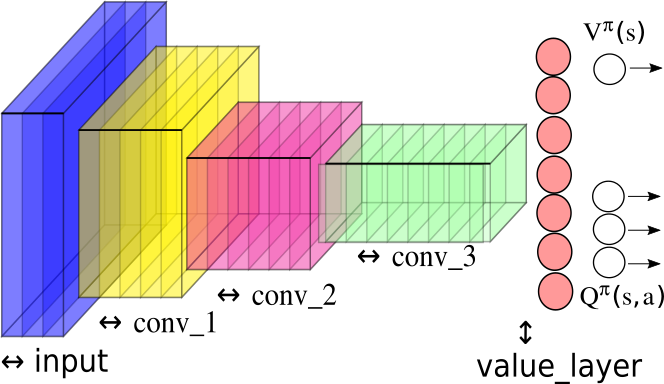
\includegraphics{./Images/Chapter07/DuelingDQV_shared.png}} \label{fig:hard_dqv}}
  \quad
  \subfloat[]{\scalebox{0.25}{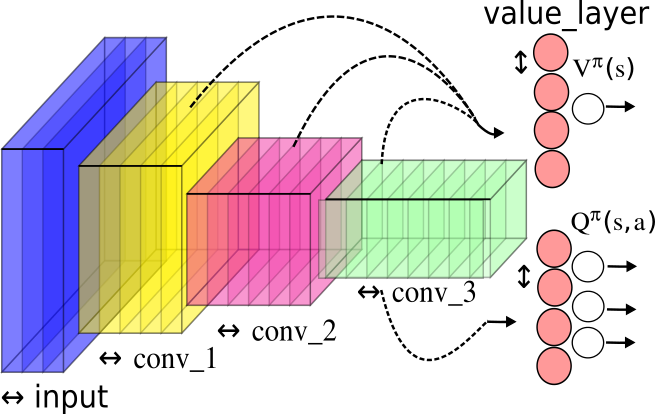
\includegraphics{./Images/Chapter07/dueling_DQV.png}} \label{fig:dueling_dqv}}
  }
\caption{Two representations of convolutional neural networks which jointly approximate the $V$ function and the $Q$ function with the aim of reducing DQV's learning parameters. On the left, an architecture which simply adds one output node to the network next to the output nodes which estimate the $Q$ function. On the right an architecture in which a specific hidden layer precedes the output that is necessary for computing each value function. When it comes to the $V$ function we experiment with different locations of such hidden layer, which is positioned after each possible convolution block.}
\end{figure}

The results obtained by these alternative versions of DQV are presented in Figs. \ref{fig:hard_dqv_results}, \ref{fig:duelling_dqv_results} and \ref{fig:tiny_dqv_results} where we report the learning curves obtained by the tested algorithms on six different \texttt{Atari} games. Each DQV extension is directly compared to the original DQV algorithm. We can observe that all the extensions of DQV, which aim at reducing the number of trainable parameters of the algorithm, fail in performing as well as the original DQV algorithm. Starting from Fig. \ref{fig:hard_dqv_results} we can observe that \textit{Hard-DQV} does not only yield significantly lower rewards (see the results obtained on \texttt{Boxing}) but also presents more unstable training (as highlighted by the results obtained on the \texttt{Pong} environment). Lower rewards and unstable training also characterize the \textit{Tiny-DQV} algorithm (see results on \texttt{Bank Heist} and \texttt{Crazy Climber} reported in Fig.\ref{fig:tiny_dqv_results}). Overall the most promising extensions of DQV are its \textit{Dueling} counterparts, we have observed in particular that the best performing architecture over most of our experiments was the \textit{Dueling-DQV-3rd} one. As can be seen by the results reported in Fig. \ref{fig:duelling_dqv_results} on the \texttt{Pong} environment we can observe that \textit{Dueling-DQV-3rd} has a comparable performance to DQV, even though it converges slower. Unfortunately, \textit{Dueling-DQV-3rd} still shows some limitations, in particular when tested on more complicated environments such as \texttt{Enduro}, we can observe that it under-performs DQV with $\approx$ 200 points. It is also worth mentioning that the idea of approximating the $V$ function before the $Q$ function explored by \textit{Dueling-DQV-1st} and \textit{Dueling-DQV-2nd} yielded negative results.

\begin{figure}[ht!]
  \begin{tikzpicture}[scale = 0.65]
      \begin{axis}[
	name=ax1,
      	grid style={dashed,gray},
      	grid = both, 
      	tick style=black,
	title=Boxing,
        xlabel=Episodes,
        ylabel=Reward,
      ]


      \addlegendentry{DQV}
      \addlegendentry{Hard-DQV}
      
      \addplot [ultra thick, red, mark=.] table [y=DQV, x=episodes]
      {./Results/Chapter07/logs/hard_dqv_boxing_results.txt};
      \addplot [ultra thick, purple, mark=.] table [y=Hard-DQV, x=episodes]{./Results/Chapter07/logs/hard_dqv_boxing_results.txt};
     
      \legend{}

      \end{axis}

      \begin{axis}[
	at={(ax1.south east)},
	xshift=2cm,
      	grid style={dashed,gray},
      	grid = both, 
      	tick style=black,
	title=Pong,
        xlabel=Episodes,
        ylabel= Reward,
	legend columns=3, 
        legend style={font=\Large, at={(-0.65,-0.3,-0.4)},anchor=north west,legend columns=3},
      ]

      \addlegendentry{DQV}
      \addlegendentry{Hard-DQV}
 
      \addplot [ultra thick, red, mark=.] table [y=DQV, x=episodes]
      {./Results/Chapter07/logs/hard_dqv_pong_results.txt};
      \addplot [ultra thick, purple, mark=.] table [y=Hard-DQV, x=episodes]{./Results/Chapter07/logs/hard_dqv_pong_results.txt};
 
      \end{axis}
	\end{tikzpicture}
	\caption{}
	\label{fig:hard_dqv_results} 
\end{figure}


\begin{figure}[ht!]
  \begin{tikzpicture}[scale = 0.65]
      \begin{axis}[
	name=ax1,
      	grid style={dashed,gray},
      	grid = both, 
      	tick style=black,
	title=Pong,
        xlabel=Episodes,
        ylabel=Reward,
      ]


      \addlegendentry{DQV}
      \addlegendentry{Duelling-DQV-1st}
      \addlegendentry{Duelling-DQV-2nd}
      \addlegendentry{Duelling-DQV-3rd}

      \addplot [ultra thick, red, mark=.] table [y=DQV, x=episodes]
      {./Results/Chapter07/logs/duelling_pong_results.txt};

      \addplot [ultra thick, green, mark=.] table [y=Duelling-DQV-1st, x=episodes]{./Results/Chapter07/logs/duelling_pong_results.txt}; 
      \addplot [ultra thick, purple, mark=.] table [y=Duelling-DQV-2nd, x=episodes]{./Results/Chapter07/logs/duelling_pong_results.txt};
      \addplot [ultra thick, cyan, mark=.] table [y=Duelling-DQV-3rd, x=episodes]{./Results/Chapter07/logs/duelling_pong_results.txt};
     
    
      \legend{}

      \end{axis}

      \begin{axis}[
	at={(ax1.south east)},
	xshift=2cm,
      	grid style={dashed,gray},
      	grid = both, 
      	tick style=black,
	title=Enduro,
        xlabel=Episodes,
        ylabel= Reward,
	legend columns=4, 
        legend style={font=\Large, at={(-0.65,-0.3,-0.4)},anchor=north west,legend columns=4},
      ]

      \addlegendentry{DQV}
      \addlegendentry{Duelling-DQV-1st}
      \addlegendentry{Duelling-DQV-2nd}
      \addlegendentry{Duelling-DQV-3rd}

      {./Results/Chapter07/logs/duelling_enduro_results.txt};
      \addplot [ultra thick, red, mark=.] table [y=DQV, x=episodes]
      {./Results/Chapter07/logs/duelling_enduro_results.txt};
      \addplot [ultra thick, green, mark=.] table [y=Duelling-DQV-1st, x=episodes]{./Results/Chapter07/logs/duelling_enduro_results.txt}; 
      \addplot [ultra thick, purple, mark=.] table [y=Duelling-DQV-2nd, x=episodes]{./Results/Chapter07/logs/duelling_pong_results.txt};
      \addplot [ultra thick, cyan, mark=.] table [y=Duelling-DQV-3rd, x=episodes]{./Results/Chapter07/logs/duelling_enduro_results.txt};
     
 
      \end{axis}
	\end{tikzpicture}
	\caption{}
	\label{fig:duelling_dqv_results} 
\end{figure}


\begin{figure}[ht!]
  \begin{tikzpicture}[scale = 0.65]
      \begin{axis}[
	name=ax1,
      	grid style={dashed,gray},
      	grid = both, 
      	tick style=black,
	title=Bank Heist,
        xlabel=Episodes,
        ylabel=Reward,
      ]


      \addlegendentry{DQV}
      \addlegendentry{tiny-dqv}
      
      \addplot [ultra thick, red, mark=.] table [y=DQV, x=episodes]
      {./Results/Chapter07/logs/tiny_dqv_bankheist_results.txt};
      \addplot [ultra thick, black, mark=.] table [y=Tiny-dqv, x=episodes]{./Results/Chapter07/logs/tiny_dqv_bankheist_results.txt};
     
      \legend{}

      \end{axis}

      \begin{axis}[
	at={(ax1.south east)},
	xshift=2cm,
      	grid style={dashed,gray},
      	grid = both, 
      	tick style=black,
	title=Crazy Climber,
        xlabel=Episodes,
        ylabel= Reward,
	legend columns=2,
        legend style={font=\Large, at={(-0.65,-0.3,-0.4)},anchor=north west,legend columns=2},
      ]

      \addlegendentry{DQV}
      \addlegendentry{Hard-DQV}
 
      \addplot [ultra thick, red, mark=.] table [y=DQV, x=episodes]
      {./Results/Chapter07/logs/tiny_dqv_crazyclimber_results.txt};
      \addplot [ultra thick, black, mark=.] table [y=Tiny-dqv, x=episodes]{./Results/Chapter07/logs/tiny_dqv_crazyclimber_results.txt};
 
      \end{axis}
	\end{tikzpicture}
	\caption{}
	\label{fig:tiny_dqv_results} 
\end{figure}




\section{Discussion and Conclusion}
\label{sec:ijcnn_discussion}

We have presented two novel model-free DRL algorithms which in addition to learning an approximation of the $Q$ function also aim at learning an approximation of the $V$ function. We have compared DQV and DQV-Max Learning to DRL algorithms which only learn an approximation of the $Q$ function, and showed the benefits which come from jointly approximating two value functions over one. Our newly introduced algorithms learn significantly faster than DQN and DDQN and show that approximating both the $V$ function and the $Q$ function can yield significant benefits both in an on-policy learning setting as in an off-policy learning one. This specific training dynamic allows for a better learned $Q$ function which makes DQV and DQV-Max less prone to estimate unrealistically large $Q$ values. All these benefits come however at a price: to successfully learn two value functions, two separate neural networks with enough capacity are required. 

In the coming chapter we will analyze the transfer learning properties of convolutional neural networks that get trained with the DQN, DDQN and the newly introduced DQV-Learning algorithms.
